%==============================================================================
%  PLECTA: overlap-aware instance reconstruction of dense filament networks
%
%  Working format: Materials Characterization research article
%  (Introduction / Materials and methods / Results / Discussion / Conclusions).
%
%  Compile with:  pdflatex -> bibtex -> pdflatex x2   (or latexmk -pdf main.tex).
%  Uses only standard CTAN packages.
%
%  Open author-supplied metadata are flagged with \todo{} or \needed{}.
%==============================================================================
\documentclass[11pt,a4paper]{article}

%------------------------------- packages -------------------------------------
\usepackage[utf8]{inputenc}
\usepackage[T1]{fontenc}
\usepackage{lmodern}
\usepackage[british]{babel}
\usepackage{microtype}
\usepackage[margin=1in]{geometry}
\usepackage{amsmath,amssymb,amsfonts}
\usepackage{graphicx}
\usepackage{xcolor}
\usepackage{booktabs}
\usepackage{array}
\usepackage{siunitx}
\usepackage{caption}
\usepackage{float}
\usepackage[numbers,sort&compress]{natbib}
\usepackage{enumitem}
\usepackage{parskip}
\usepackage{url}
\usepackage[colorlinks=true,linkcolor=blue!55!black,citecolor=teal!60!black,%
            urlcolor=blue!55!black,breaklinks=true]{hyperref}

%------------------------------- style ----------------------------------------
\definecolor{fsblue}{HTML}{2B6CB0}
\definecolor{fsorange}{HTML}{DD6B20}
\definecolor{fsgreen}{HTML}{2F855A}
\definecolor{revisioncyan}{HTML}{00A6C8}
\newcommand{\rev}[1]{\textcolor{revisioncyan}{#1}}
\newcommand{\supervisorcomment}[1]{\par\smallskip\noindent%
  \textcolor{purple!75!black}{\textbf{Supervisor comment:} #1}\par\smallskip}
\captionsetup{font=small,labelfont=bf,labelsep=period}
\sisetup{detect-all,round-mode=places,round-precision=3}
\newcommand{\um}{\si{\micro\metre}}
\newcommand{\Fone}{F\textsubscript{1}}
\newcommand{\overmerge}{\textit{over-merge}}
\newcommand{\undermerge}{\textit{under-merge}}
\newcommand{\Overmerge}{\textit{Over-merge}}
\newcommand{\Undermerge}{\textit{Under-merge}}

%------------------------------------------------------------------------------
%  \todo{...} - a short reminder to ourselves about something still to be
%  settled or added before submission. Set \aqfalse to hide them all and produce
%  a clean PDF.
%------------------------------------------------------------------------------
\newif\ifaq \aqtrue
\newcommand{\todo}[1]{\ifaq{\color{fsorange}\textbf{[To do: #1]}}\fi}
\newcommand{\aq}[1]{\todo{#1}}          % older name, kept so both still work

%------------------------------------------------------------------------------
%  \needed{...} - information we do not yet have and cannot submit without.
%  Deliberately independent of the switch above so it stays visible.
%------------------------------------------------------------------------------
\newcommand{\needed}[1]{\textcolor{red}{\textbf{[Needed before submission: #1]}}}
\newcommand{\missinginfo}[1]{\needed{#1}}   % older name, kept so both still work

%------------------------------------------------------------------------------
%  \note{...} - a point to discuss between co-authors, or a section still
%  condensed that we intend to expand.
%------------------------------------------------------------------------------
\newcommand{\note}[1]{\par\smallskip\noindent\textcolor{red}{\textbf{Note:} #1}\par\smallskip}
\newcommand{\reviewnote}[1]{\note{#1}}      % older name, kept so both still work

%------------------------------------------------------------------------------
%  Generated numerical results.
%
%  results/plecta_results.tex is generated from the machine-readable PLECTA
%  records by scripts/results/make_plecta_results.py. Do not edit it directly.
%------------------------------------------------------------------------------
% Generated by scripts/results/make_plecta_results.py; do not edit.
\newcommand{\PlectaHeldoutSceneCount}{128}
\newcommand{\PlectaHeldoutFailureCount}{0}
\newcommand{\PlectaHeldoutFOneMean}{0.854}
\newcommand{\PlectaHeldoutFOneCILow}{0.845}
\newcommand{\PlectaHeldoutFOneCIHigh}{0.864}
\newcommand{\PlectaHeldoutPrecisionMean}{0.868}
\newcommand{\PlectaHeldoutPrecisionCILow}{0.858}
\newcommand{\PlectaHeldoutPrecisionCIHigh}{0.877}
\newcommand{\PlectaHeldoutRecallMean}{0.843}
\newcommand{\PlectaHeldoutRecallCILow}{0.832}
\newcommand{\PlectaHeldoutRecallCIHigh}{0.854}
\newcommand{\PlectaHeldoutRecoveryMean}{0.799}
\newcommand{\PlectaHeldoutRecoveryCILow}{0.787}
\newcommand{\PlectaHeldoutRecoveryCIHigh}{0.812}
\newcommand{\PlectaHeldoutARIMean}{0.851}
\newcommand{\PlectaHeldoutARICILow}{0.841}
\newcommand{\PlectaHeldoutARICIHigh}{0.860}
\newcommand{\PlectaHeldoutVISplitMean}{0.256}
\newcommand{\PlectaHeldoutVISplitCILow}{0.241}
\newcommand{\PlectaHeldoutVISplitCIHigh}{0.272}
\newcommand{\PlectaHeldoutVIMergeMean}{0.216}
\newcommand{\PlectaHeldoutVIMergeCILow}{0.202}
\newcommand{\PlectaHeldoutVIMergeCIHigh}{0.231}
\newcommand{\PlectaDensity20SceneCount}{32}
\newcommand{\PlectaDensity20FOneMean}{0.911}
\newcommand{\PlectaDensity20FOneCILow}{0.888}
\newcommand{\PlectaDensity20FOneCIHigh}{0.933}
\newcommand{\PlectaDensity30SceneCount}{32}
\newcommand{\PlectaDensity30FOneMean}{0.874}
\newcommand{\PlectaDensity30FOneCILow}{0.853}
\newcommand{\PlectaDensity30FOneCIHigh}{0.892}
\newcommand{\PlectaDensity40SceneCount}{32}
\newcommand{\PlectaDensity40FOneMean}{0.858}
\newcommand{\PlectaDensity40FOneCILow}{0.841}
\newcommand{\PlectaDensity40FOneCIHigh}{0.875}
\newcommand{\PlectaDensity60SceneCount}{32}
\newcommand{\PlectaDensity60FOneMean}{0.775}
\newcommand{\PlectaDensity60FOneCILow}{0.760}
\newcommand{\PlectaDensity60FOneCIHigh}{0.790}
\newcommand{\PlectaRobustnessDegradedFOneMean}{0.822}
\newcommand{\PlectaRobustnessCleanFOneMean}{0.844}
\newcommand{\PlectaRobustnessSceneCount}{50}
\newcommand{\PlectaCleanMinusDegradedFOneMean}{0.0224}
\newcommand{\PlectaCleanMinusDegradedFOneCILow}{0.0113}
\newcommand{\PlectaCleanMinusDegradedFOneCIHigh}{0.0333}
\newcommand{\PlectaDevelopmentSceneCount}{84}
\newcommand{\PlectaAblationNoGapBridgingDeltaFOne}{-0.1394}
\newcommand{\PlectaAblationSingleRoundDeltaFOne}{-0.0199}
\newcommand{\PlectaAblationNoChainExtendedFramesDeltaFOne}{-0.0215}
\newcommand{\PlectaAblationNoAnnealingDeltaFOne}{-0.0038}
\newcommand{\PlectaAblationNoCurvatureTermDeltaFOne}{-0.0046}
\newcommand{\PlectaAblationNoSubBridgeMergingDeltaFOne}{-0.0026}
\newcommand{\PlectaAblationNoJoin_PxDeltaFOne}{-0.0221}
\newcommand{\PlectaAblationNoCrossingMergingAtAllDeltaFOne}{-0.0634}
\newcommand{\PlectaAblationNoDebrisAbsorptionDeltaFOne}{-0.0021}
\newcommand{\PlectaAblationChordTermOnlyDeltaFOne}{-0.0097}
\newcommand{\PlectaAblationTangentTermOnlyDeltaFOne}{-0.1858}
\newcommand{\PlectaAblationNoSpurPruningDeltaFOne}{0.0017}


\title{\vspace{-1.2cm}\bfseries \rev{PLECTA: Overlap-aware instance
reconstruction of dense filament networks from binary masks}}

\author{%
  \begin{minipage}{0.94\textwidth}
  \centering
  Oday Allan\textsuperscript{a}\quad
  Stefan Luding\textsuperscript{a}\quad
  Igor Ostanin\textsuperscript{a,}\thanks{Corresponding author:
  \texttt{i.ostanin@utwente.nl}}\\[5pt]
  {\small\textsuperscript{a}\,Multi-Scale Mechanics (MSM), Faculty of Engineering
  Technology, University of Twente, Enschede, The Netherlands}\\[4pt]
  {\small\todo{Add ORCIDs.}}
  \end{minipage}
}
\date{}

%==============================================================================
\begin{document}
\maketitle


\begin{abstract}
Many materials and tissues, including carbon-nanotube sheets, collagen and
paper, comprise overlapping strands whose arrangement influences their
effective properties. Measuring this geometry from
micrographs requires individual strands to be traced through crossings and
signal gaps, which merge distinct strands or split one strand into disconnected
fragments. We present PLECTA, a deterministic method that segments
individual strands using only a binary image whose foreground pixels mark
strand centrelines. At each junction, PLECTA selects which strand segments
continue into one another while allowing segments to terminate. It formulates
this decision as an exact maximum-weight partial-matching problem, with an
explicit penalty for unpaired segments and no restriction on the number of
segments entering a junction. The output permits crossing pixels to belong to
multiple strands. On synthetic scenes, PLECTA resolved strand identities
more accurately than three released alternatives at every density tested. The
same ranking held on an independently published generator run at its own
settings. A separate stage
uses the corresponding greyscale micrograph to estimate which strand lies on
top at each crossing. The
complete workflow is demonstrated on scanning electron micrographs of
carbon-nanotube sheets, from raw images to individual strand instances with
estimated crossing order, without manual annotations for training or as
pipeline inputs.


\end{abstract}

\noindent\textbf{Keywords:} \rev{filament networks; instance segmentation;
graph matching; geometric reconstruction; carbon nanotubes; scanning electron
microscopy.}

\section{Introduction}
\label{sec:intro}

\begin{figure}[!t]
  \centering
  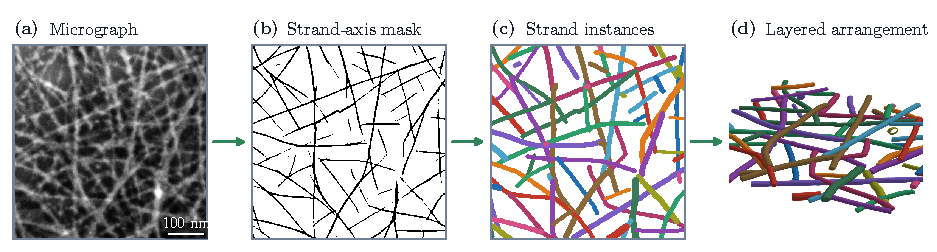
\includegraphics[width=\linewidth]{figures/fig_graphical_abstract.pdf}
  \caption{From micrograph to individual strands, on one carbon-nanotube SEM
    field held out of the segmenter's training data. \textbf{(a)} A fixed
    central crop. \textbf{(b)} The strand-axis mask from the upstream
    segmenter. \textbf{(c)} The instances PLECTA reconstructs from that mask
    alone, each drawn at the width measured for it across its own centreline.
    \textbf{(d)} The layered arrangement estimated for the same instances, at
    the same widths and without vertical exaggeration. Colour carries instance
    identity in both (c) and (d) and nothing else.}
  \label{fig:graphical-abstract}
\end{figure}

The effective properties of a strand network are influenced by the arrangement
of its individual strands, but a micrograph shows those strands only as an
overlapping tangle. This paper recovers them as separate objects from a single
greyscale scanning electron micrograph, and estimates which strand lies on top
at each crossing, placing them in depth
(Figure~\ref{fig:graphical-abstract}). The problem is not specific to one
material.

Many materials comprise networks of long, overlapping strands, including
carbon-nanotube (CNT) sheets, collagen in connective tissue, paper and nonwoven
textiles. Their stiffness, strength and conductivity depend on network
geometry, constituent behaviour and inter-strand interactions. For example,
load transfer between nanotubes can limit an assembly's stiffness and strength
despite the high modulus of each tube. Predictive models therefore require
geometric inputs such as strand length, orientation, curvature and
connectivity. Bulk image measurements such as coverage and orientation do not
establish which visible segments belong to the same strand. Recovering that
identity is necessary to measure individual strands end to end.

This is an instance-segmentation problem in which the objects are long, open
curves that overlap one another. Crossings merge distinct strands into one mask
component, whereas signal gaps split one strand into fragments whose tips can
be indistinguishable from genuine ends. Reconstruction must therefore decide
which segments continue through each junction and which reconnect across a
gap. Section~\ref{sec:related} reviews existing approaches, with the
corresponding references, and their relation to the present work.

We approach this in two steps. A greyscale micrograph is first reduced to a
binary mask marking the strand axes, by a segmenter trained on synthetic image
and mask pairs, so that no micrograph has to be annotated by hand. That mask
records where the network lies, but not which segments belong to the same
strand. Here, we address the step that follows: recovering the individual
strands from that mask alone, while allowing genuine ends, reconnecting gaps
and leaving each crossing to every strand that runs through it.

PLECTA does this by jointly selecting pairs of arms, the strand
segments entering a junction, while allowing arms to remain unpaired. It
solves an exact maximum-weight \emph{partial}-matching problem at each junction,
with an explicit penalty for unmatched arms and no restriction on junction
degree. It combines this decision with geometric checks for reconnecting gaps
and updates to direction and curvature estimates as longer strands are
assembled.
Reconstruction is deterministic for fixed inputs and parameters and assumes
directional continuity, targeting semiflexible networks whose strands maintain
their direction locally through crossings.

We evaluate PLECTA on synthetic scenes and annotated scanning electron
microscopy (SEM) images of CNT sheets, using paired clean and degraded masks
to isolate the effect of mask quality. Across the evaluated datasets, PLECTA
reconstructed strand identity more accurately than the compared methods,
although performance remained sensitive to network density and mask quality.
For SEM images, an upstream segmenter supplies the strand-axis masks. A
separate stage uses the corresponding greyscale image to estimate which strand
lies on top at each crossing; this is a proof of concept for depth ordering,
not a validated three-dimensional reconstruction.
Section~\ref{sec:methods} describes the workflow and evaluation,
Section~\ref{sec:results} reports the results, and
Section~\ref{sec:conclusions} discusses conclusions and limitations.
\Igor{After this intro, i still do not have clear image on what is the contribution of the paper. "Combination of ingridients" does not sound good. Maybe some early image -- not necessarily exhaustive, but simple and schematic -- could help.}

\section{Materials and methods}
\label{sec:methods}

\subsection{Scope and workflow}
\label{sec:mm-workflow}

PLECTA turns a binary strand-axis mask into a set of overlap-aware strand
instances, as shown in the workflow diagram in Figure~\ref{fig:scope}. For
validation and comparison against a known ground truth, the mask can be
generated synthetically; masks derived from SEM images are also tested in this
paper (Sections~\ref{sec:mm-synth} and~\ref{sec:mm-real}). PLECTA then builds a graph
of arms, stubs and junction nodes and fits a tangent and curvature frame to
each stub (Section~\ref{sec:mm-graph}). It scores candidate continuations
(Section~\ref{sec:mm-cost}), solves exact partial matchings at junctions and
across admissible gaps over eight frame-refitting rounds
(Section~\ref{sec:mm-matching}), and converts the accepted links into
overlapping strand instances (Section~\ref{sec:mm-output}). Given a paired
greyscale image, downstream stages estimate strand width and render ribbons
(Section~\ref{sec:mm-stage4}) and infer depth order at crossings
(Section~\ref{sec:mm-depth}).

\begin{figure}[!ht]
    \centering
    % ---------------------------------------------------------------------------
%  Figure 1.  Drawn in TikZ, in the document's own face at the document's own
%  size, replacing the matplotlib figures/fig_pipeline_scope.pdf whose
%  generator now writes to figures/archive/.
%
%  Layout notes:
%    * Row 2 runs right to left, so the reading order over both rows is the
%      order the method runs in: graph, frames, junction matching, gap
%      bridging, output.
%    * The dashed boundary fits only the four method stages.  The input mask
%      and the output box share column 1, so fitting either would sweep the
%      rectangle over the other; with both outside, the two arrows crossing
%      the dashed edge are the method's input and output.
%    * The depth row is grey and ends at the global order; layer and height
%      bookkeeping is left to the text (Section 2.5.2).
%    * All three depth boxes sit on the top grid's own columns, so the arrow
%      from the output box down to the first of them is exactly vertical.
%
%  Requires the pk vocabulary defined in main.tex's preamble.
% ---------------------------------------------------------------------------
\begin{tikzpicture}[pk, x=1mm, y=1mm]

  % ---- the core, two rows of three ---------------------------------------
  \node[io=38mm]    (mask)   at ( 27,   0) {Binary axis mask};
  \node[stage=38mm] (graph)  at ( 81.5, 0) {Arms, stubs and\\junction nodes};
  \node[stage=38mm] (frame)  at (136,   0) {Tangent and curvature\\frame at each stub};

  \node[io=38mm]    (out)    at ( 27,  -26) {Overlapping\\instance layers};
  \node[stage=38mm] (bridge) at ( 81.5,-26) {Gated bridging\\of mask gaps};
  \node[stage=38mm] (match)  at (136,  -26) {Exact partial matching\\at each junction};

  \draw[flow] (mask)   -- (graph);
  \draw[flow] (graph)  -- (frame);
  \draw[flow] (frame)  -- (match);
  \draw[flow] (match)  -- (bridge);
  \draw[flow] (bridge) -- (out);

  % ---- the round schedule, drawn as the cycle it is ----------------------
  \draw[loop] (bridge.north) -- (graph.south);

  % ---- the evaluated boundary -------------------------------------------
  \begin{scope}[on background layer]
    \node[scope, fit=(graph)(frame)(match)(bridge)] (core) {};
  \end{scope}

  % ---- the depth stage ----------------------------------------------------
  %  Centred to the right of the output arrow's x so the two never cross.
  \node[ext=38mm] (cross) at ( 27,  -52) {Crossings in\\projection};
  \node[ext=38mm] (ou)    at ( 81.5,-52) {Over or under,\\from brightness};
  \node[ext=38mm] (order) at (136,  -52) {One global order,\\cycles removed};

  \draw[flowsoft] (cross) -- (ou);
  \draw[flowsoft] (ou)    -- (order);
  \draw[flowsoft] (out.south) -- (cross.north);

\end{tikzpicture}

    \caption{Scope of PLECTA. The dashed grouping stage maps a binary axis mask
    to overlapping instances; the loop denotes eight rounds of frame refitting
    and matching. The grey branch uses a paired greyscale image to infer depth
    order without changing strand identity.}
    \label{fig:scope}
\end{figure}

\subsection{Synthetic data}
\label{sec:mm-synth}

Strand centrelines are generated as random walks with Gaussian-smoothed
angular increments, producing gradual bends with controllable curvature.
Strands are placed at random positions and orientations until their combined
full-width area reaches the target coverage of 20, 30, 40, 50 or 60\,\% of
the image area.
Each synthetic scene provides strand centrelines $\mathcal C_k$, their
corresponding pixel sets $\Omega_k$, and four image representations: a
one-pixel axis mask; a version with gaps and raster irregularities; a
full-width foreground mask; and an SEM-like greyscale image with
strand-specific brightness, gradual intensity variation, blur and background
noise. For depth evaluation (Section~\ref{sec:mm-depth}), a depth-resolved
variant assigns strand heights and radii, prevents interpenetration and
renders the scene from above. Occlusion, depth-dependent defocus and width
broadening are included, with imaging cues randomised independently so that
no single cue reliably determines crossing order.


\subsection{CNT SEM data and mask sources}
\label{sec:mm-real}

\PlectaRealFieldCountWord{} CNT-sheet SEM fields were analysed, each comprising
$1536\times1024$ pixels: B58\_100, B58\_110 and B58\_300, containing
\PlectaBFiveEightOneZeroZeroReferenceCount{},
\PlectaBFiveEightOneOneZeroReferenceCount{} and
\PlectaBFiveEightThreeZeroZeroReferenceCount{} annotated bundles, respectively.
Each strand annotation represents a visible bundle, as individual nanotubes
are unresolved at this magnification. The horizontal field width was
$1.66~\um$, corresponding to $1.08~\mathrm{nm\,px^{-1}}$. Images were acquired
using a Thermo Fisher Helios 5~UX DualBeam with an Elstar field-emission column
in immersion mode and a through-lens detector, at 2.00\,kV, 400\,pA and a
working distance of 4.3\,mm. Each frame integrated 35 passes at a dwell time
of 100\,ns with drift correction.

The first author (O.A.) and an independent second annotator each annotated
all \PlectaInterAnnotatorFieldCount{} fields using an in-house tool that permits
overlapping strand masks. Ridge snapping and spline smoothing assisted
tracing, while strand connections and suggested gap bridges required manual
decisions. Scores are reported separately against each annotator, with their
agreement discussed in
Section~\ref{sec:limitations}. Supplementary Section~S7 describes the
annotation procedure.

Two input masks were evaluated for each field: a skeletonised mask derived
from the first author's reference and an automatically generated mask from the
upstream CycleGAN/nnU-Net segmentation (Section~\ref{sec:res-qualitative})
\citep{ruehle2021workflow,isensee2021nnunet}. These inputs assess reconstruction
from manually curated and automatically extracted strand axes, respectively.
The automatic segmentation required no manual annotations for training or
inference.

Strand reconstruction was evaluated on the common centreline fragments
visible within each input mask,
using the metrics defined in Section~\ref{sec:mm-metrics}.


\subsection{PLECTA reconstruction}
\label{sec:mm-plecta}

Starting from a binary strand mask, PLECTA reconstructs individual strands by
resolving connections through junctions and across gaps. The following
subsections describe the main steps: constructing the skeleton graph, scoring
candidate connections and selecting compatible links, with iterative
refinement as longer strands are assembled. For an input mask
$M\in\{0,1\}^{H\times W}$, the output is a set of strand instances
$\{I_1,\ldots,I_N\}$, with $I_n\subseteq F=\{x:M(x)=1\}$; crossing pixels
may belong to multiple instances. Reconstruction uses the mask alone, while
subsequent width and depth estimates also use the greyscale image
(Section~\ref{sec:mm-image}).

\subsubsection{Skeleton graph and local geometry}
\label{sec:mm-graph}

PLECTA skeletonises the input mask using the Zhang--Suen thinning algorithm
\citep{zhang1984thinning} and removes short spurs. Pixels where three or more
skeleton branches meet are grouped into junction clusters, with nearby
clusters merged into a single \emph{node}. This accounts for crossings that
span several pixels or lie too close together to resolve separately. The
remaining strand segments form \emph{arms}, each with a \emph{stub} at either
end.

Each stub is characterised by its tip position, outward tangent
($\mathbf{t}$) and signed curvature ($\kappa$), estimated from a short segment
of the adjoining strand (Figure~\ref{fig:cost}a). Subscripts identify the stub,
so $\mathbf{t}_a$ and $\kappa_a$ denote the tangent and curvature of stub $a$.
Stubs with insufficient support for a reliable direction estimate are marked
as unreliable. As arms are linked into longer chains, these estimates are
updated using the additional strand geometry.

\subsubsection{Pairing cost function}
\label{sec:mm-cost}

The cost $C_{ab}$ of linking stubs $a$ and $b$ combines directional alignment,
chord alignment and curvature continuity (Equation~\ref{eq:cost};
Figure~\ref{fig:cost}). The reversal angle $\theta$, measured between
$\mathbf{t}_a$ and $-\mathbf{t}_b$, is zero when the outward tangents form a
straight continuation. The chord angles $\varphi_a$ and $\varphi_b$ measure
how far each tangent turns towards the opposite tip, penalising lateral
offset between otherwise aligned arms. The curvature mismatch
$\lvert\kappa_a+\kappa_b\rvert$ penalises changes in bending; the sum reflects
the opposite orientations of the outward frames. Gap links also incur a
penalty for tip separation $d$:
\begin{equation}
  C_{ab}=w_d\,\theta
        +w_t\,q(d)\,(\varphi_a+\varphi_b)
        +w_\ell\,\frac{d}{\ell_0}
        +30\,w_\kappa\,\lvert\kappa_a+\kappa_b\rvert,
  \qquad q(d)=\min\!\left(1,\tfrac{d}{d_0}\right),
  \label{eq:cost}
\end{equation}
where $w_d$, $w_t$, $w_\ell$ and $w_\kappa$ weight the four terms, and
$\ell_0$ normalises the gap distance. Junction links set $w_\ell=0$.

The reversal angle $\theta$ is independent of the tip-to-tip chord and remains
useful when nearby tips make the chord direction sensitive to pixel
quantisation. The factor $q(d)$ therefore reduces the chord-angle contribution
at separations below $d_0$. The weights, distance scales $\ell_0$ and $d_0$,
and curvature scaling factor of 30 are fixed parameters listed in
\supprecon{}. These costs quantify the suitability of individual connections;
the next step selects a compatible set of links.

\begin{figure}[tbp]
    \centering
    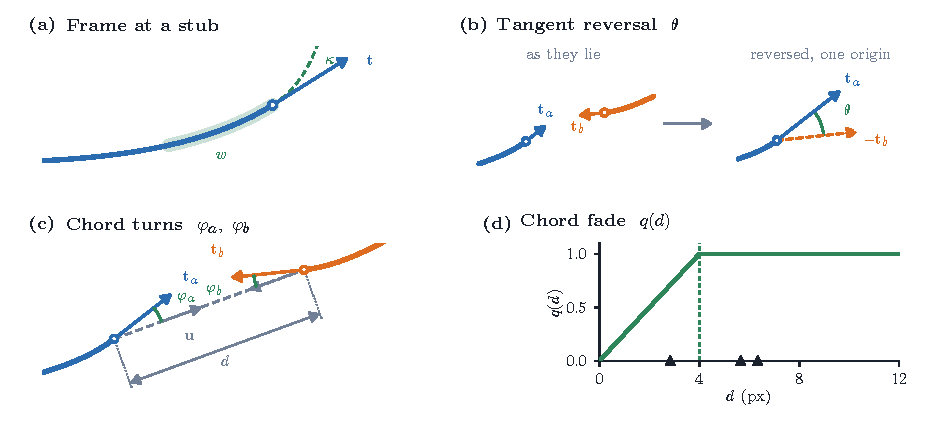
\includegraphics[width=\linewidth]{figures/fig_plecta_frame_cost.pdf}
    \caption{The stub frame and the terms of the pairing cost.
    \textbf{(a)}~The least-squares arclength fit over window $w$, read outward
    from the tip at $s=0$, giving outward tangent $\mathbf{t}$ and signed
    curvature $\kappa$; quadratic when the span allows, linear otherwise.
    \textbf{(b)}~$\theta$, in the two steps its definition takes: the outward
    tangents where they lie, then the same pair with $\mathbf{t}_b$ reversed and
    both read from one origin. A perfect continuation makes them antiparallel,
    so $\theta=0$. \textbf{(c)}~The chord turns $\varphi_a$, $\varphi_b$ onto the
    chord $\mathbf{u}$ joining the tips. \textbf{(d)}~The fade $q(d)$ against tip
    separation; triangles mark the six real separations at the crossing of
    Figure~\ref{fig:matching}.}
    \label{fig:cost}
\end{figure}

\subsubsection{Candidate selection and iterative matching}
\label{sec:mm-matching}

Using the costs from Equation~\ref{eq:cost}, PLECTA selects links jointly so
that no stub is assigned to more than one connection. Leaving stub $i$
unmatched incurs a penalty $p_i$. Connecting stubs $i$ and $j$ avoids both
unmatched penalties but incurs the linking cost $C_{ij}$ defined in
Equation~\ref{eq:cost}. The net benefit of the connection is therefore
$p_i+p_j-C_{ij}$. A link is admissible only if $C_{ij}<p_i+p_j$.
Exact maximum-weight partial matching then selects the set of disjoint stub
pairs $\Gamma$ with the greatest total benefit:
\begin{equation}
  \max_{\Gamma}\sum_{(i,j)\in\Gamma}
  \bigl(p_i+p_j-C_{ij}\bigr).
  \label{eq:matching}
\end{equation}
Each stub can belong to at most one pair or remain unmatched, allowing genuine
strand termination at junctions of any degree. The penalties therefore
determine both candidate admissibility and the preference for linking. Because
competing links are considered together, a locally favourable pair may be
rejected when another combination gives a better overall assignment.

Junction and gap links use different penalties. Gap candidates must also
satisfy distance and angular limits, since they connect strands across missing
image evidence. Figure~\ref{fig:matching} illustrates candidate selection and
matching at junctions and across gaps.

Matching proceeds iteratively, with tangent and curvature estimates updated
along the assembled chains before each round. Early rounds use lower unmatched
penalties and tighter gap-angle limits to restrict uncertain connections.
These constraints gradually relax to their configured values, and the final
round determines the output. \supprecon{} lists the penalties, geometric
limits and iteration schedule; Section~\ref{sec:res-ablation} evaluates joint
matching and the contributions of individual components.

\begin{figure}[tbp]
    \centering
    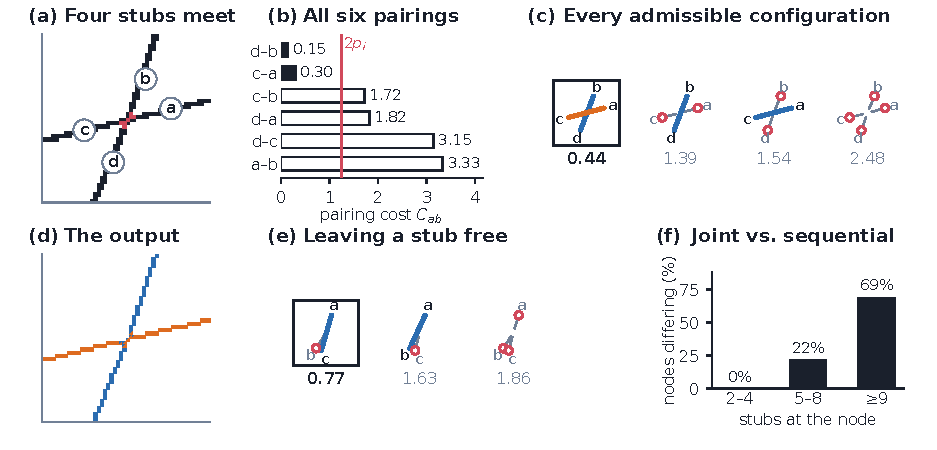
\includegraphics[width=\linewidth]{figures/fig_plecta_exact_matching.pdf}
    \caption{Candidate-link evaluation and matching outcomes, on the nodes
    where the decisions were made. Every arm is the skeleton the numbers were
    measured from, so every angle shown is the one the cost was computed on.
    \textbf{(a)}~Every pairing the admissibility gate allows at a four-arm
    crossing, each scored as a whole: its edge costs plus the penalty
    $p_i=0.62$ of each arm it leaves unmatched. The green frame marks the one
    returned; two further pairs exceed $p_i+p_j=1.24$ and are excluded as
    candidates. \textbf{(b)}~A three-arm node where an admissible edge is
    declined on the total rather than on its own cost. \textbf{(c)}~A gap link,
    which must clear all four gates at once.}
    \label{fig:matching}
\end{figure}

\subsubsection{Strand instance assembly}
\label{sec:mm-output}

After the final matching round, connected components of the accepted arm
links define individual strands. Each strand contains the pixels of its
constituent arms and associated junction clusters, allowing intersecting
strands to share crossing pixels. Accepted gap links connect fragments
belonging to the same strand without adding pixels across the gap. These
strand instances provide the input to the image-based stages described next.

\subsection{Image-informed reconstruction}
\label{sec:mm-image}

The reconstructed strands are combined with the corresponding greyscale image
to estimate their apparent widths and render ribbons
(Section~\ref{sec:mm-stage4}), and to infer crossing order
(Section~\ref{sec:mm-depth}).
These stages preserve the strand identities established during reconstruction
and do not affect the identity scores. They use fixed parameters
(\supprecon{}) and are demonstrated here on SEM images, although the procedure
accepts other greyscale images.

\subsubsection{Width and ribbon rendering}
\label{sec:mm-stage4}

Intensity profiles sampled perpendicular to each strand, away from junctions,
provide estimates of apparent width and brightness, together with uncertainty
and quality indicators. The centreline is then resampled and smoothed, with
accepted gaps interpolated, to render a ribbon at the estimated width.
Junction clusters are excluded from this rendering, and strands remain
separate. The resulting ribbons describe their projected shapes; their
relative positions in depth are estimated in Section~\ref{sec:mm-depth}.

\subsubsection{Depth ordering and height assignment}
\label{sec:mm-depth}

Depth estimation proceeds in three steps: estimating local crossing orders,
combining them into a consistent strand order, and assigning layers and heights.

\textbf{1. Estimate crossing order.} The method assumes that the upper strand
retains its brightness through a crossing, while the lower strand is occluded.
Intensity is sampled through the crossing (the \emph{core}) and along each
strand on either side (the \emph{flanks}), excluding flank pixels occupied by
the other strand (Figure~\ref{fig:depth-evidence}a,b). The pooled core median
$m_c$ is compared with the flank medians $m_i$ and $m_j$; the closer match
indicates the upper strand.

The signed score $s$ summarises this comparison
(Figure~\ref{fig:depth-evidence}c). It compares the two intensity mismatches,
normalised by the larger of $\lvert m_i-m_j\rvert$ and twice the local noise
estimate $\hat\sigma$. Its sign identifies the upper strand and its magnitude
weights the evidence. Crossings with insufficient flank samples or a score
below the threshold in magnitude remain undecided. \suppdepthstage{} gives
the sampling procedure and score equation.

\begin{figure}[!ht]
    \centering
    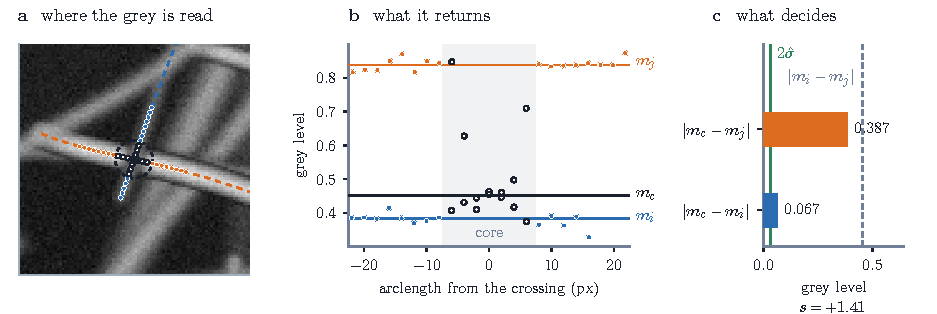
\includegraphics[width=\linewidth]{figures/fig_depth_evidence.pdf}
    \caption{Local depth evidence at a crossing angle of $83.8^{\circ}$,
    selected for clarity. Positions and intensities are taken from the stage
    output. \textbf{(a)}~Core samples (open dots) and flank samples (filled
    dots), with flanks kept clear of the other strand.
    \textbf{(b)}~Intensity along each strand: the pooled core median $m_c$
    is closer to strand $i$'s flank median than to strand $j$'s, supporting
    $i$ as the upper strand. \textbf{(c)}~Intensity mismatches used to
    calculate $s$, normalised by the larger of the flank-median separation
    and twice the local noise estimate (\suppdepthstage{}).}
    \label{fig:depth-evidence}
\end{figure}

\textbf{2. Combine crossing orders.} Local estimates can conflict: $A$ may
lie above $B$, $B$ above $C$, and $C$ above $A$. These relations form a directed
graph whose nodes are strands and whose edges carry weights $\lvert s\rvert$
(Figure~\ref{fig:depth-order}). Within each connected component, a consistent
strand order is sought with the objective of maximising the total weight of
satisfied relations. Crossing orders are updated accordingly.
\suppdepthstage{} describes the ordering procedure.

\begin{figure}[!ht]
    \centering
    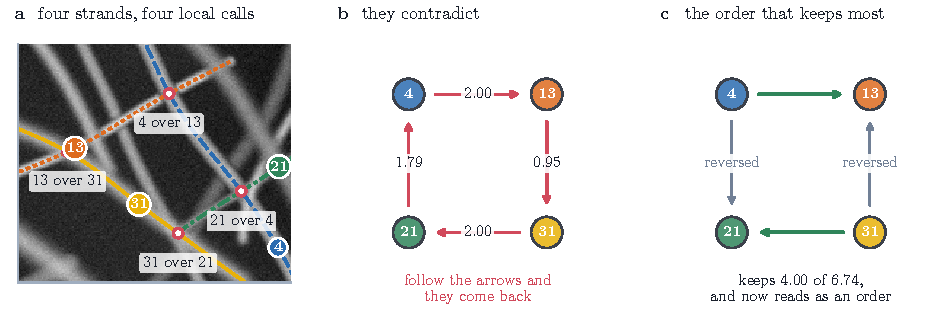
\includegraphics[width=\linewidth]{figures/fig_depth_order.pdf}
    \caption{Resolving contradictory local depth estimates.
    \textbf{(a)}~Four strands and their estimated crossing orders.
    \textbf{(b)}~The corresponding graph, with arrows from the estimated
    upper strand to the lower strand. The directed cycle prevents a
    consistent height assignment. \textbf{(c)}~The selected order retains
    the two highest-weight estimates and reverses the two lowest-weight
    estimates. Reversals are recorded with their original scores. The four
    strands shown belong to a seven-strand scene; layer assignments depend
    on the complete connected component.}
    \label{fig:depth-order}
\end{figure}

\textbf{3. Assign layers and heights.} The corrected relations form a graph
without directed cycles. Its longest path determines the minimum number of
layers needed to respect the crossing orders; strands without ordering
constraints between them may share a layer. Under the compact-stack
assumption, each strand is assigned the lowest height compatible with the
chosen order and the estimated radii, preventing interpenetration.

Without a greyscale image, placement follows the predefined tie-break rather
than measured crossing evidence. Section~\ref{sec:res-depth} evaluates depth ordering
using the measures defined in \suppdepth{}.

\subsection{Metrics and statistical analysis}
\label{sec:mm-metrics}

The primary reconstruction metric is common-fragment pairwise \Fone{}, which
measures whether strand fragments are grouped consistently with the reference.
Each input mask is divided into fragments between crossings, independently of
the reference and predictions. The same assignment rule then gives each
fragment a reference identity and a predicted identity. Pairwise precision
penalises joining fragments from different reference strands, while recall
penalises separating fragments from the same strand.
Figure~\ref{fig:f1-example} illustrates these cases and the conditions under
which the score is undefined.

\begin{figure}[!ht]
    \centering
    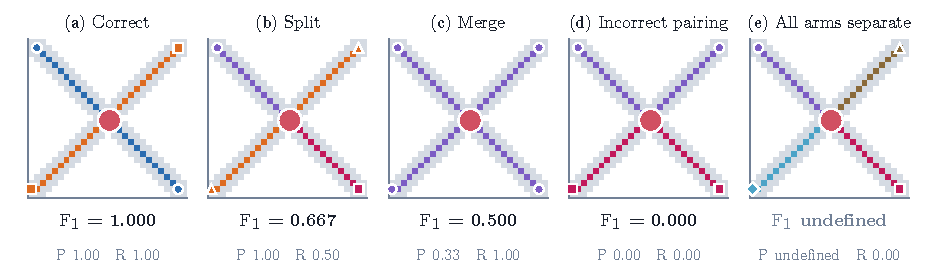
\includegraphics[width=\linewidth]{figures/fig_f1_example.pdf}
    \caption{Pairwise scoring at a crossing. Removing junction pixels (red)
    leaves four arms and six fragment pairs. Tip markers identify arms assigned
    to the same strand. \textbf{(a)}~Reference grouping.
    \textbf{(b)}~A split reduces recall. \textbf{(c)}~A merge reduces precision.
    \textbf{(d)}~Incorrect pairing changes strand identities.
    \textbf{(e)}~Separating every arm produces no predicted positive pair, so
    precision and \Fone{} are undefined.}
    \label{fig:f1-example}
\end{figure}

Because junction pixels are excluded, this metric evaluates strand continuity
through crossings rather than ownership of the crossing pixels themselves.
Strands containing more fragments contribute more pairs and therefore carry
greater weight. We also report the adjusted Rand index and variation of
information \citep{hubert1985comparing,meila2007comparing}, together with
detection \Fone{} and Crossing Fidelity, to characterise complementary aspects
of reconstruction. For the real SEM fields, Join \Fone{} evaluates joining
decisions between nearby fragments, reducing the influence of differences in
fragmentation between mask sources.

Held-out synthetic reconstruction means are accompanied by 95\,\% bootstrap
confidence intervals, with scenes resampled within each density level.
Comparisons between clean and degraded masks preserve scene pairing. For
real SEM data, each image field is treated as one independent sample.
\suppmeasures{} provides the metric definitions, assignment rules and
statistical procedures.

\section{Results}
\label{sec:results}

We first evaluate strand reconstruction on synthetic scenes
(Section~\ref{sec:res-density}), then examine depth ordering
(Section~\ref{sec:res-depth}) and application to real SEM images
(Section~\ref{sec:res-real}). Component ablations
(Section~\ref{sec:res-ablation}) and comparisons with published methods
(Section~\ref{sec:res-comparators}) assess the contributions and performance
of the reconstruction method.

\subsection{Reconstruction on synthetic images}
\label{sec:res-density}

Across the \PlectaHeldoutSceneCount{} synthetic scenes, PLECTA
achieved a mean common-fragment pairwise \Fone{} of
\PlectaHeldoutFOneMean{} (95\% bootstrap CI
[\PlectaHeldoutFOneCILow{}, \PlectaHeldoutFOneCIHigh{}]).
Table~\ref{tab:plecta-heldout} summarises reconstruction scores overall and by
areal coverage.

\begin{table}[tbp]
    \centering
    \caption{Held-out reconstruction scores overall and by target areal
    coverage. VI denotes variation of information, for which lower is better;
    higher is better for the other metrics.}
    \label{tab:plecta-heldout}
    \small
    % Generated by scripts/results/make_plecta_results.py; do not edit.
\begin{tabular}{lrrrrrrrr}
\toprule
Group & $n$ & $F_1$ & Precision & Recall & ARI & VI split & VI merge & VI total \\
\midrule
All & 128 & 0.85 & 0.87 & 0.84 & 0.85 & 0.26 & 0.22 & 0.47 \\
20\% & 32 & 0.91 & 0.93 & 0.90 & 0.91 & 0.14 & 0.09 & 0.23 \\
30\% & 32 & 0.87 & 0.89 & 0.86 & 0.87 & 0.21 & 0.16 & 0.37 \\
40\% & 32 & 0.86 & 0.86 & 0.85 & 0.85 & 0.24 & 0.22 & 0.47 \\
60\% & 32 & 0.77 & 0.79 & 0.76 & 0.77 & 0.44 & 0.39 & 0.82 \\
\bottomrule
\end{tabular}

\end{table}

Performance decreased with scene density: mean \Fone{} fell from
\PlectaDensityTwoZeroFOneMean{}
[\PlectaDensityTwoZeroFOneCILow{}, \PlectaDensityTwoZeroFOneCIHigh{}] at 20\%
coverage to \PlectaDensitySixZeroFOneMean{}
[\PlectaDensitySixZeroFOneCILow{}, \PlectaDensitySixZeroFOneCIHigh{}] at 60\%,
monotonically through the intermediate strata.
Per-scene runtime had median \PlectaHeldoutRuntimeMedian{}~s, ranging to
\PlectaHeldoutRuntimeMaximum{}~s on the densest scenes;
Section~\ref{sec:res-comparators} measures cost systematically.

PLECTA operates on the strand-axis mask, so reconstruction difficulty depends
on centreline density and geometry rather than areal coverage alone. The same
areal coverage can arise from a different centreline density under another
bundle-width distribution and may therefore produce different reconstruction
performance. Within the fixed $512\times512$-pixel frame and 7--16-pixel
bundle-width range used here, areal coverage provides a consistent within-study
stratification.

\label{sec:res-mask}%
To assess sensitivity to gaps and raster irregularities, we compared
reconstruction from clean and degraded masks of the same scenes. Across the
\PlectaRobustnessSceneCount{} synthetic scenes,
mean \Fone{} was \PlectaRobustnessDegradedFOneMean{} from degraded axes and
\PlectaRobustnessCleanFOneMean{} from the corresponding clean axes. The paired
clean-minus-degraded change was \PlectaCleanMinusDegradedFOneMean{} (95\% CI
[\PlectaCleanMinusDegradedFOneCILow{},
\PlectaCleanMinusDegradedFOneCIHigh{}]). Modelled gaps and raster
irregularities therefore caused a small reduction in reconstruction accuracy
under this generator. The difference was greatest at low coverage and narrowed
at 50--60\,\%, consistent with junction ambiguity becoming more influential
at higher density.

Figure~\ref{fig:examples} shows representative reconstructions at three
coverage levels, selected by proximity to the median \Fone{} of each stratum.

\begin{figure}[tbp]
    \centering
    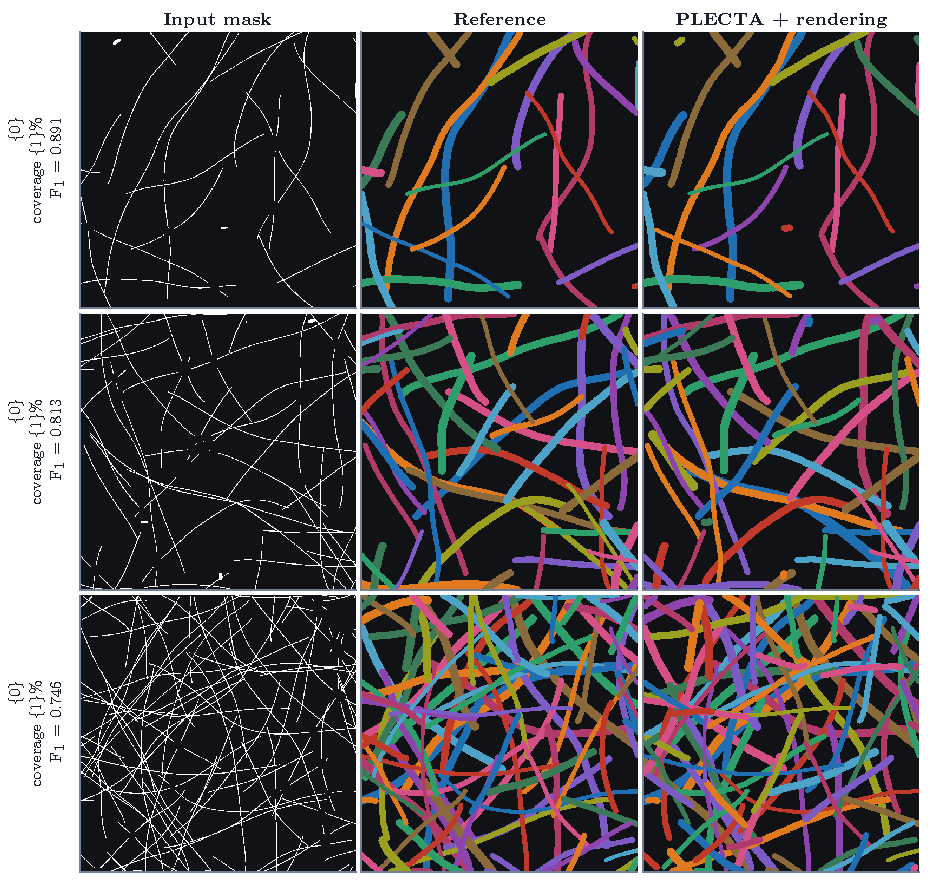
\includegraphics[width=\linewidth]{figures/fig_plecta_examples.pdf}
    \caption{Reconstruction at three coverage levels, each the scene closest
    to the median \Fone{} of its stratum, shown as a horizontal window of the
    scene. Columns: the degraded input mask, the overlap-aware reference, and
    PLECTA's strands at their fitted widths. The score beside each row is the
    grouping's, not the rendering's. Strand colours are arbitrary and not
    matched between columns.}
    \label{fig:examples}
\end{figure}

\subsection{Depth decomposition}
\label{sec:res-depth}

The stages above reconstruct strands in projection but do not establish which
strand lies above at a crossing. After grouping is fixed, the depth stage uses
the greyscale image to assess the continuity of each strand's brightness across
the crossing relative to local noise. It reconciles these local estimates into
a globally consistent vertical order and assigns non-interpenetrating heights.

The stage was evaluated on \PlectaDepthSceneCount{} depth-resolved scenes from
Section~\ref{sec:mm-synth}, at two areal coverages and under two input
conditions. Reference 2-D geometry isolates the depth decision, whereas binary
axis masks include reconstruction error. Table~\ref{tab:depth-order} reports
both using the measures defined in \suppdepth{}. Its crossing rows score local
over/under decisions before reconciliation, once for every crossing; its
stacking rows score the final order, once for every pair of strands.

\begin{table}[!ht]
\centering
\caption{The depth stage on \PlectaDepthSceneCount{} synthetic scenes whose
true vertical order is known. Chance is \PlectaDepthChance{} for every
accuracy shown.}
\label{tab:depth-order}
\begin{tabular}{lcccc}
\toprule
& \multicolumn{2}{c}{Given 2-D geometry} & \multicolumn{2}{c}{Reconstructed 2-D} \\
\cmidrule(lr){2-3}\cmidrule(lr){4-5}
Areal coverage & 20\,\% & 40\,\% & 20\,\% & 40\,\% \\
\midrule
Projected crossings per scene & 28 & 150 & 28 & 150 \\
Crossings recovered & 1.000 & 1.000 & 0.857 & 0.746 \\
Order accuracy, all crossings & 0.815 & 0.744 & 0.729 & 0.556 \\
Order accuracy, decided only & 0.890 & 0.885 & 0.961 & 0.906 \\
Abstained & 0.085 & 0.161 & 0.117 & 0.179 \\
Depth order, crossing pairs & 0.863 & 0.856 & 0.915 & 0.852 \\
Depth order, all pairs & 0.671 & 0.708 & 0.703 & 0.715 \\
Instance pairs sharing a component & 0.392 & 0.842 & 0.361 & 0.746 \\
Layer agreement & 0.656 & 0.418 & 0.702 & 0.382 \\
\bottomrule
\end{tabular}

\end{table}

Among crossings for which an order was assigned, accuracy ranged from
\PlectaDepthDecidedLow{} to \PlectaDepthDecidedHigh{} across both input
conditions and densities. The all-crossing scores were lower
(\PlectaDepthAllLow{}--\PlectaDepthAllHigh{}) because they include crossings
the 2-D stage did not recover and those for which the depth stage abstained.
The table reports recovery and abstention rates alongside these scores.

Global order is limited to evidence that can travel through the crossing graph.
Only \PlectaDepthWithinLow{} to \PlectaDepthWithinHigh{} of strand pairs lie
within the same connected component, so the relative order of the remaining
pairs is not identifiable from the available crossing evidence. All-pair order
accuracy was consequently 0.67--0.72, compared with 0.85--0.91 for pairs that
cross. Layer agreement likewise fell from \PlectaDepthCleanCovTwoZeroLayers{}
to \PlectaDepthCleanCovFourZeroLayers{} as coverage doubled, although the
recovered number of layers remained close to the reference.

Figure~\ref{fig:resem-synth} shows what the stage produces on one synthetic
scene, from the binary axis mask through to the film the reconstruction
implies; Figure~\ref{fig:resem-real} is the same sequence on a real CNT SEM
field, which no depth ground truth can score.

\begin{figure}[!ht]
\centering
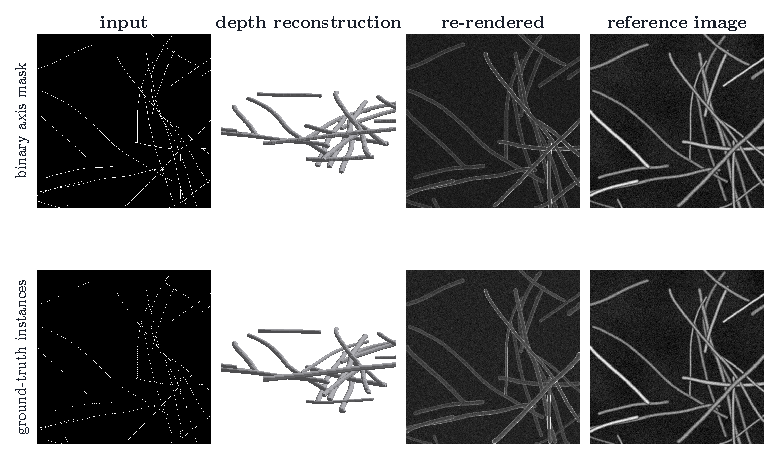
\includegraphics[width=\linewidth]{figures/fig_resem_synth.pdf}
\caption{Depth reconstruction of a synthetic scene from its binary axis mask.
The panels show the rendered greyscale image, a forward-model re-rendering from
the reconstructed depths and radii, and the inferred strand stack. The
re-rendering is a visual consistency check, not a scored quantity. The scene is
512\,px across in the generator's pixel units.}
\label{fig:resem-synth}
\end{figure}

\begin{figure}[tbp]
\centering
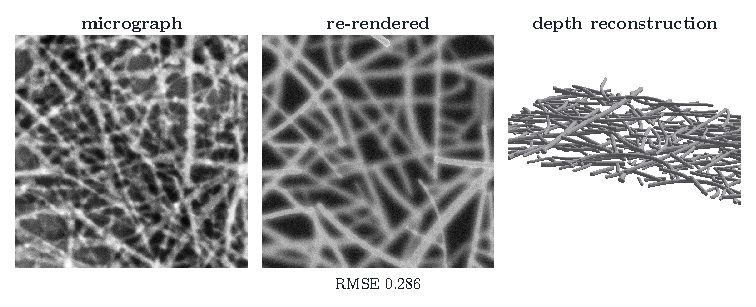
\includegraphics[width=\linewidth]{figures/fig_resem_real.pdf}
\caption{The same comparison on a real CNT SEM field, reconstructed from the
reference axis mask. The crop is 512\,px across, about 0.55\,\um{} of field
B58\_100. Real SEM provides no depth ground truth, so the depth order is shown
qualitatively; the forward-model appearance parameters are fitted to this
micrograph.}
\label{fig:resem-real}
\end{figure}

\subsection{Reconstruction on CNT SEM images}
\label{sec:res-real}
\label{sec:res-qualitative}

An upstream segmenter produces the binary strand-axis mask from each SEM
micrograph (Figure~\ref{fig:pipeline-upstream}), and PLECTA uses that mask
alone.

\begin{figure}[!ht]
    \centering
    % ---------------------------------------------------------------------------
%  Figure of Section 4.3.  Drawn in TikZ, in the document's own face at the
%  document's own size, replacing the matplotlib
%  figures/fig_pipeline_upstream.pdf whose generator now writes to
%  figures/archive/.
%
%  The upstream route is grey and the evaluated stage is not, which carries
%  the "not a contribution of this paper" distinction with line colour rather
%  than a filled region.  The training and inference clauses of the old
%  drawing live in the caption.
%
%  Requires the pk vocabulary defined in main.tex's preamble.
% ---------------------------------------------------------------------------
\begin{tikzpicture}[pk, x=1mm, y=1mm]

  % ---- training: the pair is manufactured --------------------------------
  \node[ext=32mm] (pmask)   at ( 30,   0) {Procedural\\binary mask};
  \node[ext=24mm] (gan)     at ( 79.5, 0) {CycleGAN};
  \node[ext=32mm] (semlike) at (129,   0) {SEM-like\\micrograph};

  \draw[flowsoft] (pmask) -- (gan);
  \draw[flowsoft] (gan)   -- (semlike);

  \node[ext=54mm] (corpus) at (79.5, -18)
    {Paired corpus: the procedural mask\\serves as the training label};

  \draw[flowsoft] (pmask.south)   |- (corpus.west);
  \draw[flowsoft] (semlike.south) |- (corpus.east);

  % ---- inference: the segmenter never sees an annotation -----------------
  \node[ext=32mm] (sem)    at ( 30,  -38) {Real SEM\\micrograph};
  \node[ext=24mm] (nnunet) at ( 79.5,-38) {Trained\\nnU-Net};
  \node[io=32mm]  (bmask)  at (129,  -38) {Binary strand-\\axis mask};

  \draw[flowsoft] (sem)    -- (nnunet);
  \draw[flowsoft] (nnunet) -- (bmask);
  \draw[flowsoft] (corpus.south) -- (nnunet.north);
  \node[note, anchor=west] at (82.5, -28.5) {trains};

  % ---- the stage this paper evaluates ------------------------------------
  \node[stage=32mm] (plecta) at (129, -56) {PLECTA};
  \draw[flow] (bmask) -- (plecta);

  \begin{scope}[on background layer]
    \node[scope, fit=(plecta)] (core) {};
  \end{scope}
  \node[scopelab, anchor=east, align=right] at (105, -56)
    {evaluated in this paper:\\reads that mask and nothing else};

  % ---- row labels, in the margin ------------------------------------------
  \node[note, anchor=south west] at (2,   8) {\textsc{training}};
  \node[note, anchor=south west] at (2, -31) {\textsc{inference}};

\end{tikzpicture}

    \caption{Upstream generation of the binary strand-axis mask. The segmenter
    is trained on procedurally generated image--mask pairs and requires no
    manual annotations for training or inference. Only the PLECTA stages inside
    the dashed boundary are evaluated here; the segmenter has its own
    evaluation \citep{ruehle2021workflow}.}
    \label{fig:pipeline-upstream}
\end{figure}

We evaluated \PlectaRealFieldCountLower{} manually annotated CNT-sheet fields
under two input conditions: the skeleton of the reference annotation and the
automatic nnU-Net axis \citep{ruehle2021workflow}. Both were scored against
the reference annotation, so the conditions differ only in the input mask. The
reference-derived axis tests grouping from curated real-image geometry; the
automatic axis evaluates the complete image-to-reconstruction workflow.
Figure~\ref{fig:real-sem} shows both conditions on one whole field.

\begin{figure}[tbp]
    \centering
    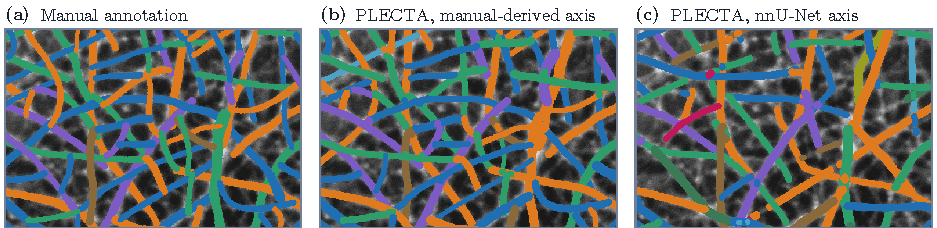
\includegraphics[width=\linewidth]{figures/fig_real_sem.pdf}
    \caption{Reconstruction of the whole B58\_110 field from two input-mask
    sources; the scale bar in (a) is 500\,nm. \textbf{(a)}~Reference
    annotation; \textbf{(b)}~reference-derived axis; \textbf{(c)}~PLECTA from
    that axis; \textbf{(d)}~automatic axis; and \textbf{(e)}~PLECTA from that
    axis with the same parameters. Input axes are dilated by one pixel for
    legibility. Predicted strands take the colour of their matched reference
    strand; crimson indicates no match.}
    \label{fig:real-sem}
\end{figure}

\begin{table}[tbp]
    \centering
    \caption{Reconstruction from reference-derived and automatic axes in three
    CNT SEM fields. Coverage is the fraction of the frame covered by full-width
    reference strands. Metrics are defined in Section~\ref{sec:mm-metrics};
    detection \Fone{} uses IoU \PlectaDetectionIoU{} and tolerance
    \PlectaPlacementTolerance{}\,px.}
    \label{tab:plecta-real-masks}
    \footnotesize
    % Generated by scripts/results/make_plecta_results.py; do not edit.
\begin{tabular}{lrllrrr}
\toprule
Field & Coverage & Input axis & Method & $F_1$ & Join $F_1$ & Det.\ $F_1$ \\
\midrule
B58\_100 & 44.0\,\% & Manual-derived & PLECTA & 0.89 & 0.93 & 0.94 \\
 &  &  & SIFNE & 0.89 & 0.92 & 0.92 \\
 &  &  & Basu$^{*}$ & 0.81 & 0.89 & 0.87 \\
 &  & U-Net & PLECTA & 0.46 & 0.56 & 0.63 \\
\addlinespace
B58\_110 & 46.7\,\% & Manual-derived & PLECTA & 0.84 & 0.91 & 0.93 \\
 &  &  & SIFNE & 0.81 & 0.89 & 0.92 \\
 &  &  & Basu$^{*}$ & 0.71 & 0.85 & 0.85 \\
 &  & U-Net & PLECTA & 0.45 & 0.59 & 0.60 \\
\addlinespace
B58\_300 & 41.5\,\% & Manual-derived & PLECTA & 0.95 & 0.96 & 0.96 \\
 &  &  & SIFNE & 0.90 & 0.94 & 0.93 \\
 &  &  & Basu$^{*}$ & 0.75 & 0.91 & 0.89 \\
 &  & U-Net & PLECTA & 0.47 & 0.62 & 0.58 \\
\bottomrule
\end{tabular}

\end{table}

Table~\ref{tab:plecta-real-masks} reports each field and condition. Mean
\Fone{} was \PlectaRealManualFOneMean{} from the reference-derived axis and
\PlectaRealUNetFOneMean{} from the automatic axis. The reference-derived
result establishes grouping on axes from real micrographs; the automatic
result measures sensitivity to the input mask. With only
\PlectaRealFieldCount{} fields, these results are descriptive and the field is
the independent sample.

The automatic axes were thicker, displaced and more fragmented than the
reference-derived axes (Figure~\ref{fig:real-sem}), and the additional errors
were mainly missed links rather than erroneous mergers. Join \Fone{} narrows
but does not remove the difference between the conditions. On B58\_110, for
example, the automatic axis gave join precision
\PlectaJoinBFiveEightOneOneZeroUNetPrecision{} and recall
\PlectaJoinBFiveEightOneOneZeroUNetRecall{}.

These three fields cannot separate segmentation error from annotation
ambiguity. Replacing the automatic axis with the independent annotation's
skeleton gave \Fone{}=\PlectaInterAnnotatorBOnAFOneMean{} against the
reference, within the direct inter-annotator agreement range of
\PlectaInterAnnotatorAgreeFLow{}--\PlectaInterAnnotatorAgreeFHigh{}. The
automatic-axis result should therefore be interpreted alongside annotation
ambiguity, as discussed in Section~\ref{sec:limitations}.

\subsection{Development ablations}
\label{sec:res-ablation}

Component contributions were evaluated by removing one component at a time
and rescoring, together with two controls that are not components of the
method. All ablations are measured on the development scenes.

\textbf{Contribution of each component.} Table~\ref{tab:plecta-ablation} varies one
thing at a time. Two rows change what a link costs, dropping the junction
chord-turn term or the curvature term; two change the graph the linker reads,
leaving neighbouring junction clusters unconsolidated or arms too short to
merge the crossings they join; two change the iteration, running a single
round or removing the schedule that relaxes the gates; and one removes gap
bridging, so identity never crosses a break in the mask. The three largest
losses are the junction chord-turn term, gap bridging and junction-cluster
consolidation.

Two rows are controls rather than components. The greedy control retains
all other PLECTA components but pairs each node's arms in ascending order of
edge cost, rather than by whichever complete pairing of that node is cheapest
overall; an early low-cost selection can preclude a later mutually compatible
pairing, thereby causing fragmentation rather than erroneous merging. It also runs at parameters that were selected using the exact
matcher, a bias in the exact matcher's favour. The last row replaces the
linker outright, skeletonising the same mask and greedily pairing the branch
ends that turn least inside fixed distance and angle gates, which is the
pairing principle shared by SIFNE, GraFT's path cover and Wegmayr et
al.\ \citep{zhang2017sifne,osterlund2026graft,wegmayr2020microplastic}.

\begin{table}[tbp]
    \centering
    \caption{Component ablations and the two controls, on development scenes.
    The three blocks use different scene sets, so $n$ is given per row and
    each $\Delta F_1$ is against PLECTA on that row's own scenes; the column is
    not comparable across rows of different $n$.}
    \label{tab:plecta-ablation}
    \small
    % Generated by scripts/results/make_plecta_results.py; do not edit.
\begin{tabular*}{\linewidth}{@{\extracolsep{\fill}}lrrr@{}}
\toprule
Variant & $F_1$ & $\Delta F_1$ & ARI \\
\midrule
Fixed configuration & 0.87 & +0.000 & 0.86 \\
No joint junction solve & 0.78 & -0.080 & 0.77 \\
No gap bridging & 0.73 & -0.139 & 0.72 \\
Single round & 0.85 & -0.020 & 0.84 \\
No chain-extended frames & 0.85 & -0.021 & 0.84 \\
No round schedule & 0.86 & -0.004 & 0.86 \\
No curvature term & 0.86 & -0.005 & 0.86 \\
No short-connector node merging & 0.85 & -0.022 & 0.84 \\
No junction-cluster consolidation & 0.80 & -0.063 & 0.80 \\
No junction chord-turn term & 0.68 & -0.186 & 0.67 \\
Whole linker replaced & 0.68 & -0.145 & 0.67 \\
\bottomrule
\end{tabular*}

\end{table}


\subsection{Published methods on identical masks}
\label{sec:res-comparators}

PLECTA was compared with four published methods on two data sets: the
\PlectaGreedySceneCount{} synthetic scenes the comparison was designed on, and
the \PlectaRealFieldCountLower{} annotated CNT SEM fields of
Section~\ref{sec:res-real}, where the manual-derived axis lets the same
comparison run on real imaging. All four are scored beside PLECTA on identical masks, through the same
conversion and metric code, over scenes generated after every configuration
was fixed. What is compared is narrow: the
overlap-aware grouping of a binary axis mask of dense, crossing strands, at
the coverages and tangling of the scenes described in
Section~\ref{sec:mm-synth}. Each of these methods was built for a different
setting, and how it performs in that setting is not what these numbers
measure. DNAi \citep{playout2026dnai}, GraFT \citep{osterlund2026graft} and
SIFNE \citep{zhang2017sifne} are run from their own released sources. For the
fourth, \citet{basu2015extraction}, no implementation was found, and it is
reimplemented here. Adapting each method to a common input and evaluation pipeline required
methodological choices, and each of those choices is stated here.


\begin{table}[!ht]
    \centering
    \caption{PLECTA against four published methods, identical masks and one
    scorer, ordered by \Fone{}. The upper block is the degraded synthetic
    scenes; the lower is the annotated CNT SEM
    fields of Section~\ref{sec:res-real} on the manual-derived axis, a plain
    mean over the \PlectaRealFieldCountLower{}. Variation of
    information in bits, lower better; higher better for the rest.\\[2pt]
    $^{*}$\,our reimplementation; no implementation of that paper was found.
    \suppcomparators{} details it.}
    \label{tab:plecta-comparators}
    \small
    % Generated by scripts/results/make_plecta_results.py; do not edit.
\begin{tabular}{lrrrrr}
\toprule
Measure & PLECTA & Greedy & DNAi & GraFT & PLECTA $-$ greedy \\
\midrule
Common-fragment $F_1$ & 0.822 & 0.676 & 0.343 & 0.490 & +0.145 [+0.129, +0.162] \\
Precision & 0.831 & 0.785 & 0.462 & 0.666 & +0.046 [+0.029, +0.062] \\
Recall & 0.814 & 0.599 & 0.284 & 0.400 & +0.215 [+0.196, +0.235] \\
Reference-instance recovery & 0.765 & 0.542 & 0.252 & 0.304 & +0.223 [+0.201, +0.245] \\
Adjusted Rand index & 0.817 & 0.670 & 0.331 & 0.479 & +0.148 [+0.131, +0.165] \\
Variation of information~$\downarrow$ & 0.573 & 1.036 & 2.107 & 1.558 & -0.463 [-0.509, -0.418] \\
\addlinespace
Crossings resolved exactly & 0.809 & 0.729 & 0.581 & 0.683 & +0.065 [+0.047, +0.083] \\
Resolution index & 0.778 & 0.736 & 0.401 & 0.639 & --- \\
\addlinespace
Median s per scene, 20/60\% & 0.14--4.1 & --- & 0.04--0.6 & 2.44--29.7 & --- \\
\bottomrule
\end{tabular}

\end{table}

\textbf{How each was run.} Each released method has a front end that precedes
the stage assigning identity, and in each case the mask is injected where that
stage begins, so grouping is not confounded with segmentation and all
identity-assignment stages run the original authors' code. Each was also run at a configuration
selected on the same \PlectaDevelopmentSceneCount{} development scenes PLECTA
was configured on rather than at its own defaults. These adaptations favour the comparators, and by a wide margin: run end to
end on the greyscale, GraFT scores \PlectaGraFTNativeFOne{} against
\PlectaGraFTFOne{} injected, and reconfiguration increased \Fone{} from
\PlectaDNAiShippedFOne{} to \PlectaDNAiFOne{} for DNAi and from
\PlectaSifneShippedFOne{} to \PlectaSifneFOne{} for SIFNE. Both are
reported.
\suppcomparators{} gives each injection point, each selection, what was not
attempted, and how each method fails.

\begin{figure}[!t]
  \centering
  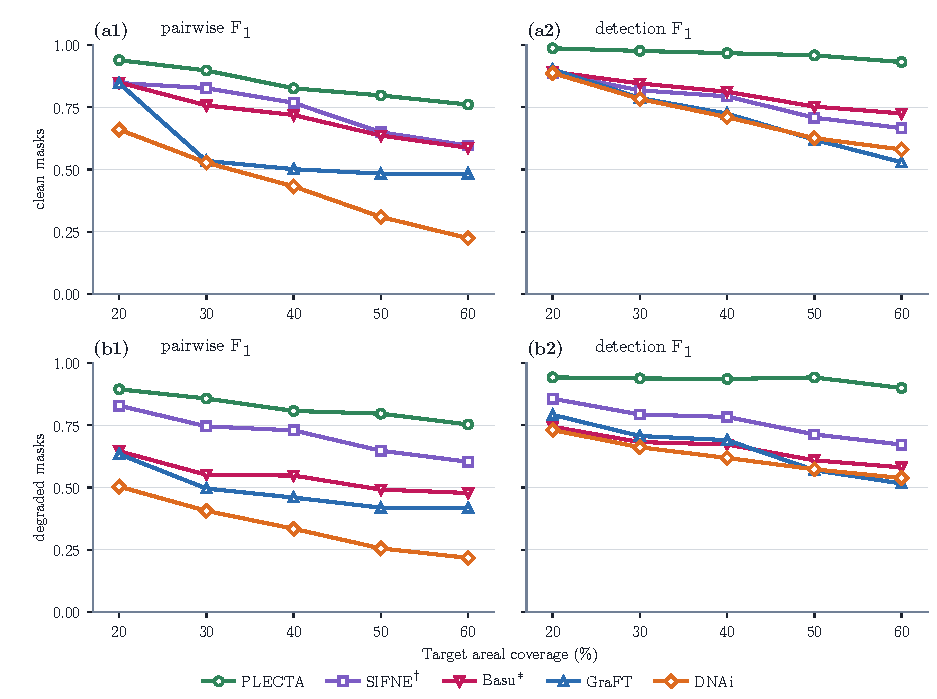
\includegraphics[width=\linewidth]{figures/fig_metric_panels.pdf}
  \caption{Five methods on identical masks, by coverage stratum. Rows: the
    undegraded axis, panels \textbf{(a)} and \textbf{(b)}, above the
    degraded one, panels \textbf{(c)} and \textbf{(d)}. Columns: pairwise
    \Fone{}, which counts pairs of fragments, and detection \Fone{} at IoU
    \PlectaDetectionIoU{} with a
    \PlectaPlacementTolerance{}\,px tolerance, which counts objects
    (Section~\ref{sec:mm-metrics}). The two disagree where a method
    fragments, since only the first is quadratic in fragmentation. Crossing
    Fidelity is in Table~\ref{tab:plecta-comparators}. Means of ten scenes.
    $^{*}$\,our reimplementation; none was found.}
  \label{fig:metric-panels}
\end{figure}

Under these comparator-favouring settings, the ranking of
Table~\ref{tab:plecta-comparators} remained constant across density levels
and mask conditions (Figure~\ref{fig:metric-panels}). SIFNE is the
strongest of them, so the margin is measured against a method configured for
this data rather than against an unsuitable default. Two entries qualify that ordering. The first is
DNAi, whose deficit is a limitation of domain and density rather than a
general ranking: it is built for DNA-fibre micrographs, which are sparse, and
where the network is sparse and the axis clean it recovers
\PlectaDNAiCleanSparseFOne{} at 20\% coverage. The second is
\citet{basu2015extraction}, the closest structural relative PLECTA's junction
matching has in that it too optimises over a neighbourhood and penalises
joins by curvature. It stands second only to PLECTA on Crossing Fidelity while its
pairwise \Fone{} is substantially below both released methods, so the curvature-priced
matching is effective at the junctions, and the deficit arises in the
stages around that decision. That is why the unmatched-arm penalty of
Section~\ref{sec:mm-plecta} is claimed as part of a combination rather than
on its own. \suppcomparators{} gives both in full.

\textbf{Each method in its own regime.} That ordering is drawn from one
generator, so it was tested in the regimes the two released methods were built
for. On GraFT's own generator, run unmodified at its published settings over
\PlectaRegimeSceneCount{} scenes in \PlectaRegimeStratumCount{} density
strata, PLECTA achieved the highest \Fone{} at every density and no rank
reversals occurred, including inside the range GraFT itself published, and
the field-standard measures order the three identically. Overall it
achieved
\Fone{}=\PlectaRegimeOverallPlectaFOne{} there, against
\PlectaRegimeOverallGraFTFOne{} for GraFT on its own scenes and
\PlectaRegimeOverallDNAiFOne{} for DNAi. SIFNE released no generator, so the sparse cobweb
topology its paper validates against was rebuilt here from that description;
on that reconstruction the two methods are level in the regime the SIFNE
publication addresses,
\PlectaSifneOwnSparsePlectaFOne{} against \PlectaSifneOwnSparseSifneFOne{},
and separate only slightly at the denser end. That places the difference in
the degree of crossing entanglement rather than in the total strand content
of the frame,
though a topology we rebuilt is weaker evidence than a generator its authors
released. \suppcomparators{} gives both density series in full.


\textbf{Cost.} The methods differ in computational cost as well as in
accuracy. Per-scene cost was measured warm, single-threaded and pinned to
one core, timing each method's own computation only
(Table~\ref{tab:plecta-comparators}). These
are independently optimised codebases, so absolute times measure
implementation as much as algorithm.

\textbf{On real imaging.} The two comparators that read a binary axis were run
over the \PlectaRealFieldCountLower{} annotated fields as well, on the
manual-derived masks of Section~\ref{sec:res-real} and through the same
scoring pipeline as PLECTA on those fields.
Averaged over the \PlectaRealFieldCountLower{}, PLECTA achieved
\Fone{}=\PlectaRealManualFOneMean{}, against \PlectaRealSifneFOneMean{} for
SIFNE and \PlectaRealBasuFOneMean{} for Basu, and the highest value on every
measure reported. The ordering established on synthetic scenes therefore holds on
masks read off real micrographs.

The margin is narrower than on the synthetic scenes, which likely reflects
the quality of the manually derived axes: a skeleton of a hand annotation is
unbroken, thin and placed where a person judged the strand to be, so it
contains few of the fragmentation and displacement artefacts responsible for
the differences observed in the synthetic evaluation.

\section{Conclusions}
\label{sec:conclusions}
\label{sec:discussion}
\label{sec:limitations}

Micrographs of strand networks show crossings that merge distinct strands and
gaps that split one strand into fragments, so each strand's identity is lost
in the image. Recovering it is what makes per-strand length, orientation and
curvature measurable. PLECTA recovers it from a binary image marking strand
centrelines alone, deciding at each junction which segments continue into one
another and allowing a strand to end rather than be forced onward. Crossing
pixels are assigned to every strand passing through them. PLECTA's grouping
core requires no training data and produces identical output from identical
input masks. The upstream segmenter is trained on synthetic image--mask pairs,
so the full workflow requires no manually annotated training micrographs.

\begin{itemize}[leftmargin=1.5em,label=\textbullet,topsep=6pt,itemsep=2pt,parsep=0pt]
  \item Across \PlectaHeldoutSceneCount{} synthetic scenes, PLECTA achieved a mean
        pairwise \Fone{} (agreement on whether two fragments belong to the
        same strand) of \PlectaHeldoutFOneMean{} [\PlectaHeldoutFOneCILow{},
        \PlectaHeldoutFOneCIHigh{}], falling from
        \PlectaDensityTwoZeroFOneMean{} to \PlectaDensitySixZeroFOneMean{} as
        areal coverage, the fraction of the frame the strands fill, rises from 20
        to 60\,\%.
  \item With every method given the same input mask, PLECTA achieved the highest
        scores among the evaluated methods across the tested densities. Its lead
        was also retained on GraFT's released generator at published settings.
  \item The ablation analysis identified the junction term penalising turning, and
        the reconnection of fragments across signal gaps, as the largest
        contributors to segmentation performance.
  \item The greyscale depth stage ordered the crossings it did not decline with
        \PlectaDepthDecidedLow{}--\PlectaDepthDecidedHigh{} accuracy, against
        chance level \PlectaDepthChance{}. Its global order is limited to
        strands connected through crossings.
\end{itemize}

\noindent\textbf{Scope and limitations.}

\begin{itemize}[leftmargin=1.5em,label=\textbullet,topsep=6pt,itemsep=2pt,parsep=0pt]
  \item PLECTA assumes directional continuity through crossings and remains
        sensitive to upstream mask errors. It can bridge short gaps but cannot
        recover omitted strands or reliably correct false axes.
  \item The real-material evaluation is a case study of
        \PlectaRealFieldCountLower{} CNT SEM fields. The automatic-axis mean
        \Fone{} of \PlectaRealUNetFOneMean{} lies within the range over which
        two human annotators agree with each other,
        \PlectaInterAnnotatorAgreeFLow{}--\PlectaInterAnnotatorAgreeFHigh{},
        so it should be interpreted alongside ambiguity in defining strand
        identity through local occlusions.
  \item The comparisons test all methods on the same binary masks in the
        dense, crossing networks studied here. They show PLECTA's advantage in
        this setting, but do not assess each method in the imaging application
        for which it was originally developed.
\end{itemize}

\noindent\textbf{Outlook.}

\begin{itemize}[leftmargin=1.5em,label=\textbullet,topsep=6pt,itemsep=2pt,parsep=0pt]
  \item \textbf{Improved binary segmentation.} A more accurate upstream segmenter,
        trained on synthetic data better matched to real micrographs, would
        improve the masks PLECTA receives.
  \item \textbf{Validation on real data.} CNT sheets stacked in a known order, or
        focused-ion-beam cross-sections of the imaged region, would give the true
        crossing order for the depth stage; a real development set, kept separate
        from the evaluation fields, would let parameters be tuned on imaging rather
        than on synthetic scenes alone.
  \item \textbf{Broader application.} Other materials, magnifications and SEM
        applications.
  \item \textbf{Mechanical models.} The segmented strands, with their depth order
        and widths, can serve as input geometry for mesoscale mechanical
        simulations.
\end{itemize}

\section{Conclusions}
\label{sec:conclusions}

FilaSeg reconstructs overlapping filament instances from degraded centreline
masks through deterministic Hough vectorization, orientation-aware cleaning and
geometric reconnection. On \LockedSceneCount{} predefined procedural scenes, its
Stage-3 centreline output achieved common-fragment \Fone{} of
\LockedFilaSegCommonFOneMean{} (density-stratified 95\% CI
[\LockedFilaSegCommonFOneCILow{}, \LockedFilaSegCommonFOneCIHigh{}]). The paired
difference from the fixed minimum-turn comparator was
\FilaSegMinusBaselineSkeletonCommonFOneMean{} (95\% CI
[\FilaSegMinusBaselineSkeletonCommonFOneCILow{},
\FilaSegMinusBaselineSkeletonCommonFOneCIHigh{}]).

The evaluator audit changed the scientific interpretation without changing any
frozen method output. Equivalent Stage-3 centrelines are the defensible primary
grouping representation; Stage-4 centreline changes and width-rendered masks are
secondary diagnostics. Automatically selected counterexamples show that the
aggregate advantage is not uniform across scenes or densities. The result is
therefore evidence for this fixed comparison under the tested generator, not a
claim of superiority over filament tracing methods generally.

The single real crop remains a development illustration. Independent real
annotations from multiple parent images, complete acquisition and annotation
metadata, separate validation of apparent width and other exported
measurements, and a citable clean-checkout release are required before broader
SEM or quantitative microstructure claims are justified.


%------------------------------- back matter ----------------------------------
\section*{CRediT author contribution statement}
\todo{Fill in each author's CRediT roles before submission, checked against
actual contributions; keep the author names and order as listed above.}

\section*{Declaration of competing interest}
The authors declare that they have no known competing financial interests or
personal relationships that could have appeared to influence the work reported
in this paper.

\section*{Data and code availability}
\rev{The frozen implementation, configuration, seed manifest, evaluation
scripts, and machine-readable results are available at
\url{https://github.com/Jorallan/PLECTA}. Generated scene images remain local
because they are procedurally reproducible from the recorded seeds.}
\todo{Create a tagged archival release and add its DOI before submission; do
not infer or preassign a DOI.}

\section*{Acknowledgements}
\rev{The authors thank the maintainers of NumPy, SciPy, scikit-image, NetworkX,
and Matplotlib. The upstream synthetic-data-driven mask workflow adapts the
open CycleGAN/U-Net particle-segmentation workflow of Rühle et
al.~\citep{ruehle2021workflow}; it is not evaluated as the contribution of this
paper.}

\bibliographystyle{unsrtnat}
\bibliography{references}

\end{document}
